% total_main.tex -- the eight section files inlined into one document, generated by
% scripts/flatten_paper.py.  Everything else (main.tex's preamble, style/, the .bib files, figure/) is
% unchanged and still required to build.  Edit the section files, not this one: regenerate it instead,
% or the next regeneration silently discards the edits.
%
\documentclass{article} % For LaTeX2e
% Target venue: ICLR 2027.  The kit under style/ is the 2025 one from the IGDM release; drop the
% 2027 .sty/.bst into style/ and change the two lines naming them.  Nothing else depends on the
% year.  Layout: this file + N_Section.tex are the manuscript, style/ is the venue kit, *.bib the
% bibliography, notes/ the prose companions that are NOT part of the build.
% 2026-09-05: the `times` option requests the ptm family, which has no TU (unicode) shapes under
% this engine, so every shape fell back to LM Roman regular and \textbf, \emph and \textsc were
% silently rendering as regular text -- paragraph headings and bold table rows included.  Forcing T1
% takes the legacy path, where ptm has its full set of shapes.
\usepackage[T1]{fontenc}
\usepackage{style/iclr2025_conference,times}

% Optional math commands from https://github.com/goodfeli/dlbook_notation.
\input{style/math_commands.tex}

\usepackage{hyperref}
\usepackage{url}

%%%%%%%%%%%%%%%%%%%%%%%%%%%%%% ADD PACKAGES %%%%%%%%%%%%%%%
\usepackage{subcaption}
\usepackage{amsmath}
\usepackage{amssymb}
\usepackage{amsthm}
\usepackage{cleveref}
\usepackage{booktabs}
\usepackage{multirow}
\newcommand{\ie}{\emph{i.e.}}

\usepackage{algorithm}
\usepackage{algorithmic}

\usepackage{array}
% FLOAT PLACEMENT (2026-09-05).  Every table was declared [t] and there are seven in the experiments
% section alone, so LaTeX ran out of top slots, deferred them, and dumped the queue at the end of the
% document -- tab:ladder and tab:controls were landing on page 25 of a 13-page body.  Widening the
% float parameters gives the placement algorithm room, and placeins puts a barrier at each section so
% a float can no longer cross out of the section that declares it.
\usepackage[section]{placeins}
\setcounter{topnumber}{3}
\setcounter{bottomnumber}{2}
\setcounter{totalnumber}{4}
\renewcommand{\topfraction}{0.92}
\renewcommand{\bottomfraction}{0.6}
\renewcommand{\textfraction}{0.06}
\renewcommand{\floatpagefraction}{0.7}
\usepackage{sidecap}
\usepackage{xcolor}   % [table] dropped: another package loads xcolor first, and we use no row colours

\usepackage{textgreek}
\usepackage{tikz}
\usepackage{wrapfig}

\setlength{\aboverulesep}{0.6pt}
\setlength{\belowrulesep}{1.5pt}

% Propositions and proofs were running into the surrounding prose and were hard to find when
% skimming.  amsthm's plain style (bold header, italic body) plus a little air around the environment
% is enough; an earlier version drew a rule down the left margin, which read as a quote block.
\theoremstyle{plain}
\newtheorem{proposition}{Proposition}
\newtheorem{corollary}{Corollary}
\makeatletter
\def\thm@space@setup{%
  \thm@preskip=1.4\parskip \@plus 3pt \@minus 1pt
  \thm@postskip=\thm@preskip}
\makeatother

% Run-in headings carry the structure of the experiments section, so give them room to be seen.
\makeatletter
\renewcommand{\paragraph}{\@startsection{paragraph}{4}{\z@}%
  {1.8ex \@plus 0.7ex \@minus .2ex}{-0.7em}%
  {\normalfont\normalsize\bfseries}}
\makeatother
\newcommand{\dg}{\textsuperscript{\dag}}
\newcommand{\ddg}{\textsuperscript{\ddag}}
%%%%%%%%%%%%%%%%%%%%%%%%%%%%%%%%%%%%%%%%%%%%%%%%%%%%%%%%%%%%

% Title framing note: an earlier version ended "...without a Robust Teacher", which invites the
% reading "so with a robust teacher you lose" -- and we would, since IGDM+AdaAD reaches
% 64.44/30.32 on this architecture from a WRN-28-10 teacher.  That is a ranking claim against a
% line this paper does not compete with.  The register here follows B-MTARD and ARREST, whose
% titles both name the goal ("Mitigating the Accuracy-Robustness Trade-off") and the mechanism,
% and claim nothing about what is unnecessary.
\title{Clean Feature Anchoring: Mitigating the Accuracy--Robustness\\
Trade-off by Self-Distilling a Naturally Trained Model}

\author{
Anonymous authors\\
Paper under double-blind review
}

\newcommand{\fix}{\marginpar{FIX}}
\newcommand{\new}{\marginpar{NEW}}

% \iclrfinalcopy   % uncomment only for the camera-ready; submissions must stay anonymous

\begin{document}

\maketitle

%% ============================================================================
%% 0_Abstract.tex
%% ============================================================================
\begin{abstract}
Adversarial training improves robustness but often sacrifices accuracy on
clean data, leading to a persistent clean--robust trade-off. We address this
trade-off by first learning a high-accuracy clean self-teacher exclusively
from natural images and then preserving its clean knowledge while
adversarially training the student. We propose Clean Feature Anchoring (CFA),
which matches the student's adversarial representation to the fixed clean
representation of the self-teacher while retaining its classifier, requiring
no label-based objective during adversarial training.

We connect predictive distillation to direct regression onto a fixed clean
target and show that, for the feature-space realization, controlling the
anchor jointly bounds clean teacher--student discrepancy and local feature
variation. We further find that teacher clean accuracy alone does not
determine how much clean performance is retained after robust transfer. To
account for example-dependent responses to perturbations, we additionally
allocate a fixed batch budget of attack radii according to the local
sensitivity of the anchoring objective. On CIFAR-100 with ResNet-18,
sensitivity matching improves clean accuracy by \(2.19\) percentage points on
average across three runs while leaving AutoAttack accuracy nearly unchanged.
CFA achieves \(64.82\mathbin{\pm}0.07\%\) clean accuracy and
\(28.04\mathbin{\pm}0.09\%\) AutoAttack accuracy, with consistent results
across CIFAR-10, Tiny-ImageNet, and WideResNet-34-10.
\end{abstract}

\section{Introduction}
\label{sec:intro}

Adversarial training is one of the most effective approaches to improving
robustness against adversarial perturbations, but this robustness often comes
at the cost of accuracy on clean data
\citep{PGD,tsipras2018robustness,TRADES}. This clean--robust trade-off raises
a natural question: can a model acquire robustness while retaining more of
the representation that supports strong clean performance?

We approach this problem by separating the learning of clean knowledge from
the learning of robustness. Before adversarial training, we first train a
clean self-teacher exclusively on natural images, allowing it to learn a
high-accuracy clean representation without adversarial perturbations. We then
initialize a student from this model and adversarially train the student while
preserving the knowledge encoded by the clean self-teacher. The role of the
teacher is therefore not to provide robustness. Instead, it provides a clean
reference that the student seeks to retain while learning robustness.

This perspective differs from conventional robust distillation, which often
transfers knowledge through predictive distributions and balances
distillation against label-based supervision \citep{ard,rslad,adr,bmtard}.
We instead ask whether the clean knowledge of the self-teacher can serve
directly as a fixed target throughout the student's adversarial neighborhood.
This leads to \textbf{Clean Feature Anchoring (CFA)}, in which the student's
adversarial representation is matched to the clean representation of the
self-teacher while the inherited classifier remains fixed. The
adversarial-training stage therefore requires no label-based objective: the
clean self-teacher defines what should be preserved, while adversarial
perturbations define the neighborhood over which it should be preserved.

\begin{figure}[t]
  \centering
  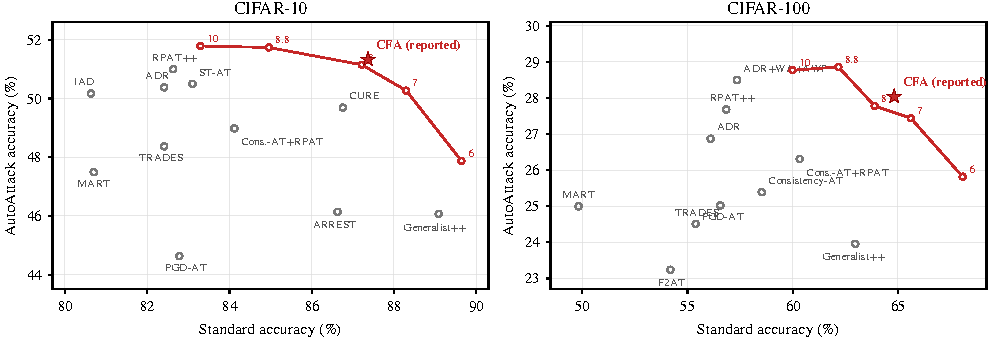
\includegraphics[width=\linewidth]{figure/frontier.pdf}
  \caption{Clean--AutoAttack trade-off on CIFAR-10 and CIFAR-100 with
  ResNet-18 at \(\epsilon=8/255\). Grey points are published results
  (\Cref{tab:published}); the CFA curve varies the training radius over
  100-epoch runs, and the star denotes the reported 150-epoch result trained
  at \(\epsilon_{\mathrm{train}}=8/255\).}
  \label{fig:frontier}
\end{figure}

We study this formulation from two complementary perspectives. First, we
examine how the clean self-teacher should supervise the robust student.
Increasing the temperature of predictive distillation connects softened
prediction matching to regression onto a fixed clean logit target. This
motivates direct clean-target regression and places CFA as its feature-space
realization. Feature and logit regression reach similar empirical operating
points, suggesting that the broader mechanism is the use of a fixed clean
target rather than an inherent advantage of feature coordinates. For the
feature realization, we further show that controlling a single clean anchor
simultaneously bounds the student's discrepancy from the clean teacher and
its local feature variation, without requiring the teacher itself to be
robust.

Second, we examine what determines the clean knowledge that is transferred.
A teacher with higher clean accuracy does not necessarily yield a student
with higher clean accuracy after adversarial training, and teachers with
nearly identical clean accuracy can transfer substantially different clean
performance. These observations indicate that teacher clean accuracy alone
is an incomplete description of transferability.

The fixed clean target specifies what the student should preserve, but a
uniform perturbation radius treats all training examples identically in input
space. The same radius, however, need not induce a comparable change in the
anchoring objective for every example. We therefore introduce
sensitivity-matched perturbation budgets, which redistribute a fixed batch
budget according to the local sensitivity of the anchor loss. This
complements clean feature anchoring: the self-teacher determines the reference
representation, while sensitivity matching determines the neighborhood over
which each example is trained to preserve it.

Empirically, CFA improves the clean--robust trade-off across CIFAR-10,
CIFAR-100, and Tiny-ImageNet, and extends to WideResNet-34-10. On CIFAR-100
with ResNet-18, CFA achieves \(64.82\mathbin{\pm}0.07\%\) clean accuracy and
\(28.04\mathbin{\pm}0.09\%\) AutoAttack accuracy across three runs.
Sensitivity matching improves clean accuracy by \(2.19\) percentage points on
average over a uniform-radius counterpart while leaving AutoAttack accuracy
nearly unchanged.

Our contributions are summarized as follows:
\begin{itemize}
  \item We introduce a clean self-teacher framework for mitigating the
  clean--robust trade-off, in which clean knowledge is learned before
  adversarial training and subsequently preserved through a fixed clean
  target. CFA instantiates this principle in feature space without a
  label-based objective during adversarial training.
  \item We characterize fixed clean-target transfer both theoretically and
  empirically. High-temperature predictive distillation connects to fixed
  clean-logit regression, while the feature-space realization jointly
  controls clean teacher--student discrepancy and local feature variation.
  We further show that teacher clean accuracy alone is insufficient to
  characterize robust transfer.
  \item We introduce sensitivity-matched perturbation budgets that
  redistribute a fixed batch budget according to the local response of the
  anchoring objective, improving clean accuracy without an observed loss in
  robustness in the final CIFAR-100 configuration.
\end{itemize}

\section{Related Work}
\label{sec:related}

\paragraph{Adversarial training and its targets.}
PGD adversarial training optimizes a model on worst-case inputs \citep{PGD}; TRADES separates clean
prediction from local consistency \citep{TRADES}, and MART reweights misclassified examples
\citep{MART}. Subsequent work improves generalization through label smoothing, consistency
regularization, weight averaging, and adversarial weight perturbation
\citep{pang2020bag,tack2022consistency,robustoverfit,2020_awp}. ADR replaces one-hot labels with
targets produced by an annealed momentum teacher \citep{adr}. These approaches motivate our study
of how the supervisory target affects the clean--robust trade-off.

\paragraph{Predictive targets in adversarial distillation.}
ARD transfers a robust teacher's predictions during adversarial training \citep{ard}. RSLAD emphasizes
robust soft labels \citep{rslad}, IAD discounts unreliable teacher guidance \citep{iad}, and AdaAD uses
the teacher in both adversarial-example generation and student optimization \citep{adaad}. IGDM adds
the teacher's local input geometry to logit-based distillation \citep{igdm}. These methods are designed
to inherit robustness from an adversarially trained teacher. Our target instead comes from a natural
teacher at the clean input and remains fixed during the student's inner maximization.

\paragraph{Guidance from naturally trained models.}
BGAT is the closest direct-regression precedent: it matches adversarial logits to a fixed natural
teacher's clean logits, and LBGAT extends this to a jointly trained natural branch \citep{lbgat}.
Our logit control confirms that this fixed-clean-target principle is not specific to features. CFA
uses the full clean representation with an inherited fixed classifier, and our analysis focuses on
what a fixed clean anchor controls, how teacher properties relate to transferability, and how its
perturbation neighborhood is allocated. ARREST starts
from a naturally pretrained model and regularizes latent representations while retaining adversarial
cross-entropy and noisy replay \citep{arrest}. HAT uses a natural helper to label examples outside the
training ball \citep{hat}, and B-MTARD combines clean and robust teachers with adaptive temperature
and loss balancing \citep{bmtard}.

\paragraph{Sample-dependent perturbation budgets.}
IAAT and CAT adapt the training radius to sample difficulty, while MMA directly increases an
input-space margin \citep{iaat,cat,mma}. Our allocation has a different source: it redistributes a
fixed batch budget according to the input sensitivity of the loss being optimized. The comparison is
therefore not between adaptive and uniform radii alone, but between the signals used to assign the
same budget.

%% ============================================================================
%% 2_Analysis.tex
%% ============================================================================

\section{Analysis}
\label{sec:analysis}

Adversarial training often improves robustness at the cost of clean accuracy.
To mitigate this trade-off, we first learn a clean self-teacher exclusively
from natural images and then transfer its knowledge while adversarially
training the student. A central question is therefore how this clean
knowledge should be transferred under adversarial perturbations. We first
revisit predictive distillation and its high-temperature behavior, then move
to a fixed clean target and study the feature-space realization used by CFA.
We subsequently characterize what the anchor controls and examine how teacher
clean performance relates to transferability.

\subsection{From Predictive Distillation to a Fixed Clean Target}
\label{sec:fragile}

Let \(f=h\circ\Phi\), where \(\Phi\) is a feature map and
\(h(z)=Wz+b\) is a linear classifier. Subscripts \(t\) and \(s\) denote the
frozen clean self-teacher and student. Given a clean input \(x\) and a
perturbed input \(x'\in B(x,\epsilon)\), shared-temperature distillation uses
\begin{equation}
q_t^\tau(x)=\operatorname{softmax}(f_t(x)/\tau),\qquad
p_s^\tau(x')=\operatorname{softmax}(f_s(x')/\tau),
\end{equation}
and minimizes
\(\tau^2D_{\rm KL}(q_t^\tau(x)\|p_s^\tau(x'))\).
Increasing \(\tau\) makes both predictive distributions progressively softer.
Although the probabilities approach the uniform distribution, their scaled
discrepancy retains the relative structure of the underlying logits.

More precisely, for fixed logits and
\(\bar f=f-C^{-1}\mathbf1\mathbf1^\top f\),
\begin{equation}
\lim_{\tau\to\infty}\tau^2D_{\rm KL}(q_t^\tau(x)\|p_s^\tau(x'))
=\frac{1}{2C}\|\bar f_t(x)-\bar f_s(x')\|_2^2.
\label{eqn:kd_limit}
\end{equation}
The centering reflects the shift invariance of softmax: adding the same
constant to every logit leaves the predictive distribution unchanged. Thus,
high-temperature predictive distillation approaches direct regression of the
perturbed student's logits onto the clean teacher's logits, up to a common
shift.

This connection motivates a more direct view of knowledge transfer. Rather
than passing clean knowledge through a softened predictive distribution, the
student can be regressed directly onto a fixed clean target. CFA applies this
principle at the representation level:
\begin{equation}
\mathcal L_{\rm anchor}(x)=\max_{x'\in B(x,\epsilon)}
\|\Phi_s(x')-\Phi_t(x)\|_2^2.
\label{eqn:anchor_percell}
\end{equation}
Here, \(\Phi_t(x)\) is computed once from the clean input and serves as the
fixed target, whereas the student is optimized against the worst-case
perturbed input. Feature matching is a design choice rather than a
mathematical consequence of \Cref{eqn:kd_limit}; logit regression constrains
the representation through the classifier output, while feature regression
directly constrains the representation supplied to the inherited classifier.

\begin{figure}[t]
  \centering
  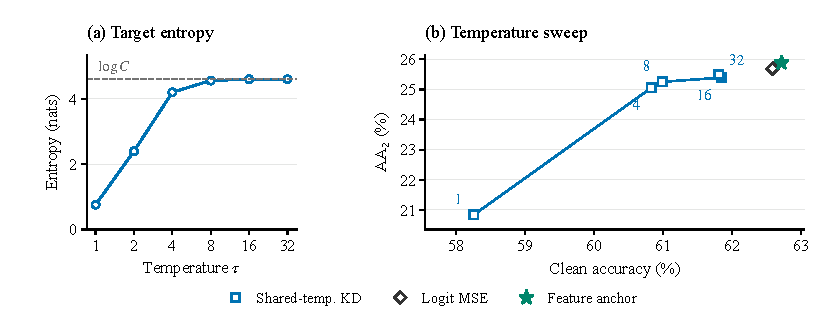
\includegraphics[width=\linewidth]{figure/analysis_targets.pdf}
  \caption{Target comparison on CIFAR-100 (ResNet-18). (a) Entropy of the
  clean teacher target as the shared temperature increases. (b) Clean accuracy
  and AutoAttack (AA) under shared-temperature knowledge distillation (KD), direct logit regression, and feature
  regression. Exact values are in \Cref{tab:targetcomparison_values}.}
  \label{fig:targetcomparison}
\end{figure}

As shown in \Cref{fig:targetcomparison}, increasing the shared temperature
moves KD toward the operating point obtained by direct logit regression,
consistent with \Cref{eqn:kd_limit}. Direct feature regression is close to
logit regression rather than decisively better; the same remains true under
the final training stack (\Cref{tab:finalallocation,tab:regression_stack}).
The comparison therefore supports fixed clean-target regression as the broader
mechanism without establishing an inherent empirical advantage of feature
coordinates.

A second distinction is where the teacher is evaluated. The natural teacher's
feature can change substantially inside the perturbation ball, so asking the
student to match the teacher at the perturbed input can reproduce precisely
the behavior that the robust stage should avoid. Under the same 50-epoch
control, the fixed clean target \(\Phi_t(x)\) reaches \(61.33\%\) clean and
\(26.19\%\) AA, whereas replacing it with \(\Phi_t(x_{\rm adv})\) raises
clean accuracy to \(76.11\%\) but collapses AA to \(0.00\%\)
(\Cref{tab:teacherread}). Thus the teacher supplies the clean reference value
to preserve, rather than a perturbed response to imitate. We next characterize
what controlling this fixed anchor implies for the student.

\subsection{What the Anchor Controls}
\label{sec:decomp}

CFA is designed to preserve the representation of the clean self-teacher while
the student is trained against adversarial perturbations. For
\(B=B(x,\epsilon)\), define
\begin{equation}
L=\max_{x'\in B}\|\Phi_s(x')-\Phi_t(x)\|_2,\quad
F=\|\Phi_s(x)-\Phi_t(x)\|_2,\quad
O=\max_{x',x''\in B}\|\Phi_s(x')-\Phi_s(x'')\|_2.
\label{eqn:LFO}
\end{equation}
Here, \(L\) is the worst-case discrepancy from the fixed clean anchor and is
the quantity directly controlled by CFA. \(F\) measures clean
teacher--student fidelity, while \(O\) is the diameter of the student's
feature set over the perturbation region.

\begin{proposition}[Fixed-anchor decomposition]\label{prop:decomp}
For every \(x\) and \(\epsilon\ge0\),
\begin{equation}
L\le F+O\le3L.
\label{eqn:decomp}
\end{equation}
\end{proposition}
The argument is short and exposes why a single anchor controls both terms.
Because \(x\in B(x,\epsilon)\), we immediately have \(F\le L\). Moreover,
for any \(x',x''\in B(x,\epsilon)\), the triangle inequality gives
\begin{equation}
\|\Phi_s(x')-\Phi_s(x'')\|_2
\le \|\Phi_s(x')-\Phi_t(x)\|_2
   + \|\Phi_s(x'')-\Phi_t(x)\|_2
\le 2L,
\end{equation}
so \(O\le2L\); the other direction, \(L\le F+O\), follows by inserting
\(\Phi_s(x)\) between \(\Phi_s(x')\) and \(\Phi_t(x)\). Hence
\(L\le F+O\le3L\). The complete proof and scope are given in
\Cref{app:anchor_scope}. In particular, if \(L\le\delta\), then
\(F\le\delta\) and \(O\le2\delta\): keeping the worst-case student feature
close to the clean teacher anchor simultaneously preserves clean-teacher
fidelity and limits local feature variation. This conclusion does not require
the clean teacher itself to be robust or locally stable; only its
representation at the clean input serves as the anchor.

Because CFA inherits the teacher's linear classifier, the same discrepancy
also limits deviation at the classifier output:
\begin{equation}
\|h_t(\Phi_s(x'))-h_t(\Phi_t(x))\|_2
\le \|W_t\|_{2\rightarrow2}\,L.
\end{equation}
This bound does not by itself guarantee identical predictions, which also
depend on the teacher's clean classification margin. The fixed-anchor argument
is also not specific to feature coordinates and analogously applies to
norm-based regression onto a fixed logit target. It characterizes the joint
control induced by a fixed target rather than establishing an inherent
advantage of feature matching. Finite-step PGD only approximates the inner
maximum and therefore does not certify the true value of \(L\).


\subsection{Does Better Clean Teacher Performance Transfer to the Student?}
\label{sec:teacher_transfer}

The preceding analysis shows how a fixed clean representation can serve as an
anchor for the adversarially trained student. This raises a natural question
about the source of that target: does improving the clean performance of the
self-teacher also improve the clean performance transferred to the student?

\begin{figure}[!htbp]
  \centering
  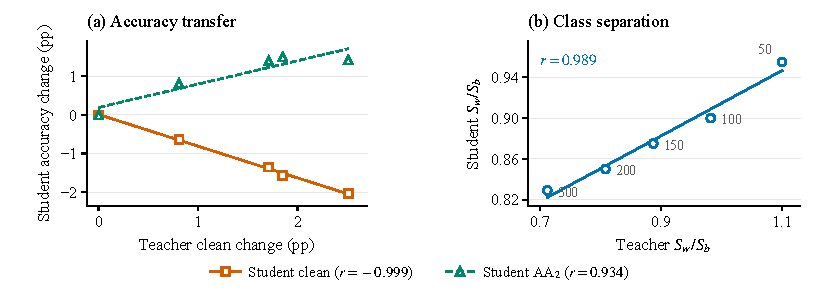
\includegraphics[width=\linewidth]{figure/teacher_checkpoint_trends.pdf}
  \caption{
  Transfer from clean self-teachers at different stages of training on
  CIFAR-100 (ResNet-18).
  (a) Changes in teacher clean accuracy and resulting student clean accuracy
  and AA relative to the 50-epoch teacher.
  (b) Within-to-between scatter ratios $S_w/S_b$ of teacher and student
  features; lower values indicate stronger class separation, and labels
  denote teacher epochs. Lines are least-squares fits; exact values are
  reported in \Cref{tab:teacherladder_values}.
  }
  \label{fig:teacherladder}
\end{figure}

Along one CIFAR-100 teacher trajectory, teacher clean accuracy rises from
\(75.81\%\) at 50 epochs to \(78.32\%\) at 300 epochs. This improvement does
not translate into higher student clean accuracy: the corresponding student
accuracy falls from \(64.28\%\) to \(62.24\%\), while AA rises from
\(24.38\%\) to \(25.80\%\) (\Cref{fig:teacherladder}). The relationship is
not strictly monotonic on the robust axis either, since the 200-epoch teacher
produces slightly higher AA than the 300-epoch teacher. An independently
trained teacher trajectory shows the same overall pattern
(\Cref{tab:teacherladder_seed1}). Higher teacher clean accuracy therefore
leads to different clean--robust operating points rather than being directly
inherited as student clean accuracy.

Teacher clean accuracy also does not reveal what changes in the transferred
representation as training progresses. The within-to-between scatter ratio
\(S_w/S_b\), measured on unit-normalized clean features, decreases for both
teacher and student along the trajectory (\Cref{fig:teacherladder}). This
association indicates that changes in teacher representation are reflected in
the resulting student, but does not identify which representational property
causes the observed clean--robust shift.

We further compare two clean self-teachers trained with label smoothing and
mixup that have nearly identical clean accuracy. Despite differing by only
\(0.14\) percentage points in teacher clean accuracy, they produce students
whose clean accuracies differ by \(4.18\) points, while AA differs by only
\(0.02\) points (\Cref{tab:matchedteacher}). Taken together, these results
distinguish teacher clean performance from transferability: clean accuracy is
an incomplete descriptor of the representation being transferred rather than
a sufficient criterion for selecting a teacher. For the remaining
experiments, we fix the 200-epoch checkpoint as a reference teacher and hold
it constant.

\section{Method}
\label{sec:method}

The preceding analysis motivates two design choices. First, the clean
self-teacher provides a fixed representation target, allowing the student to
preserve the teacher's clean representation while controlling its variation
under perturbations. Second, even with the teacher fixed, a uniform
input-space radius need not induce a comparable change in the anchoring
objective across examples. Based on these observations, CFA combines clean
feature anchoring with sample-dependent perturbation budgets.

\subsection{Clean Feature Anchoring}
\label{sec:anchor}
Let \(\Phi_t,h_t\) denote the frozen clean self-teacher. The student inherits
\(\Phi_s\leftarrow\Phi_t\) and \(h_s=h_t\), after which only \(\Phi_s\) is
optimized. For each clean example,
\begin{equation}
 x_{\rm adv}=\arg\max_{x'\in B(x,\epsilon)}
 \|\Phi_s(x')-\Phi_t(x)\|_2^2,\qquad
 \mathcal L_{\rm CFA}=\mathbb E_x\|\Phi_s(x_{\rm adv})-\Phi_t(x)\|_2^2.
\label{eqn:anchor}
\end{equation}
We approximate the inner maximization with randomly initialized PGD. No label
loss is used in this stage, and inference uses \(h_t\circ\Phi_s\). The full
procedure is given in \Cref{alg:cfa}.

\subsection{Sensitivity-Matched \(\epsilon\)}
\label{sec:angeps}
A uniform pixel radius can induce different changes in the anchor loss across
examples. For
\(\ell_{\rm anc}(x';x_i)=\|\Phi_s(x')-\Phi_t(x_i)\|_2^2\), first-order
movement in an \(\ell_\infty\) ball satisfies
\begin{equation}
\max_{\|\delta\|_\infty\le e}\langle\nabla_{x'}\ell_{\rm anc},\delta\rangle
=e\|\nabla_{x'}\ell_{\rm anc}\|_1.
\label{eqn:firstorder}
\end{equation}
Motivated by this relation, let \(g_i>0\) be a local sensitivity score for
example \(x_i\). We assign smaller perturbation radii to more sensitive
examples and larger radii to less sensitive ones according to
\begin{equation}
\epsilon_i=N\epsilon\frac{g_i^{-p}}{\sum_{j=1}^N g_j^{-p}},
\label{eqn:angeps_ideal}
\end{equation}
where \(p\) controls the strength of sensitivity matching. The case \(p=0\)
recovers a uniform radius, while larger \(p\) increasingly redistributes the
budget according to sensitivity. By construction,
\(\sum_i\epsilon_i=N\epsilon\), so the procedure changes only how the
perturbation budget is distributed across examples rather than the average
strength of adversarial training. Unlike sample weighting in the outer
objective, it changes each example's perturbation neighborhood while retaining
equal weight in the training average.

The first-order relation motivates sensitivity as the allocation signal; it
does not imply that nonlinear adversarial losses are exactly equalized. We
therefore test the assignment empirically against a uniform radius and against
controls that preserve or replace the radius distribution while changing
which examples receive each radius (\Cref{tab:allocation}). Implementation
details, clipping, and the sensitivity-norm control are reported in
\Cref{app:box}.

\section{Experiments}
\label{sec:exp}

We evaluate CFA with three questions in mind: how it compares with existing adversarial training and robust distillation methods, whether its behavior generalizes across datasets and architectures, and whether the proposed anchor and radius allocation account for the resulting clean--robust trade-off.

\subsection{Experimental Settings}
We evaluate CIFAR-10, CIFAR-100 \citep{krizhevsky2009learning}, and Tiny-ImageNet-200 \citep{le2015tiny}, using ResNet-18 as the default architecture and WideResNet-34-10 to test model-scale transfer. Unless stated otherwise, the clean self-teacher is trained on natural images for 200 epochs and then frozen. The student is initialized from this teacher, with the inherited classifier kept fixed during adversarial training. Main CIFAR runs use 150 epochs, AdamW, a one-cycle schedule, 10-step projected gradient descent (PGD-10), \(\epsilon_{\rm train}=8/255\), sensitivity matching (\(p=1\)), weight averaging (WA), and adversarial weight perturbation (AWP).

We compare with standard adversarial training and robust distillation baselines using their respective training recipes; distillation baselines receive the same natural teacher where applicable. We report clean and AutoAttack (AA) accuracy on the full test set at \(8/255\), together with their arithmetic mean (Avg) and harmonic mean (denoted NRR). Dataset-specific settings, teacher statistics, attack diagnostics, and additional controls are provided in \Cref{app:repro,app:gradmask}.

\subsection{Main Results}
\begin{table}[!htbp]
  \centering
  \footnotesize
  \setlength{\tabcolsep}{3.2pt}
  \caption{
  ResNet-18 results under \(\ell_\infty\) perturbations with
  \(\epsilon=8/255\). All values are measured in our framework.
  \emph{T.} denotes the teacher assumed by each method: none (--),
  a natural model (nat.), or the method's own weight average (self).
  The CIFAR-100 CFA row reports the mean of three student seeds;
  all other rows are individual runs.
  }
  \label{tab:main}
  \begin{tabular}{llrrrrrrrr}
    \toprule
    & & \multicolumn{4}{c}{CIFAR-10}
      & \multicolumn{4}{c}{CIFAR-100} \\
    \cmidrule(lr){3-6}\cmidrule(lr){7-10}
    Method & T. & Clean & AA & Avg & NRR
           & Clean & AA & Avg & NRR \\
    \midrule
    PGD-AT & -- & 84.54 & 43.57 & 64.06 & 57.50
                 & 57.36 & 20.34 & 38.85 & 30.03 \\
    TRADES & -- & 81.71 & 49.16 & 65.44 & 61.39
                 & 55.28 & 23.55 & 39.42 & 33.03 \\
    MART   & -- & 80.41 & 45.56 & 62.99 & 58.16
                 & 53.86 & 22.72 & 38.29 & 31.96 \\
    \midrule
    ARD & nat. & 84.58 & 43.75 & 64.16 & 57.67
               & 57.61 & 20.24 & 38.93 & 29.96 \\
    RSLAD & nat. & 85.15 & 42.91 & 64.03 & 57.06
                 & 59.68 & 21.30 & 40.49 & 31.40 \\
    AdaAD & nat. & 85.39 & 46.22 & 65.81 & 59.98
                 & 59.79 & 23.19 & 41.49 & 33.42 \\
    AdaAD + IGDM & nat. & 85.01 & 45.50 & 65.26 & 59.27
                        & 48.25 & 19.48 & 33.87 & 27.75 \\
    LBGAT & nat. & -- & -- & -- & --
                 & 56.46 & 26.02 & 41.24 & 35.62 \\
    ARREST & nat. & 85.06 & 46.42 & 65.74 & 60.06
                  & \textbf{66.97} & 22.78 & 44.88 & 34.00 \\
    \midrule
    HAT & nat. & 84.59 & 48.81 & 66.70 & 61.90
               & 60.67 & 24.45 & 42.56 & 34.85 \\
    ADR & self & 83.36 & 49.72 & 66.54 & 62.29
               & 59.93 & 27.20 & 43.57 & 37.42 \\
    RPAT++ & -- & 82.41 & 50.75 & 66.58 & 62.82
                  & 55.93 & 27.36 & 41.64 & 36.74 \\
    \midrule
    \textbf{CFA (ours)}
      & nat.
      & \textbf{87.37} & \textbf{51.33}
      & \textbf{69.35} & \textbf{64.67}
      & \textbf{64.82} & \textbf{28.04}
      & \textbf{46.43} & \textbf{39.15} \\
    \bottomrule
  \end{tabular}
\end{table}

On CIFAR-100, CFA reaches \(64.82\%\) clean and \(28.04\%\) AA (NRR
\(39.15\)); relative to ADR, the closest baseline in NRR, this is
\(+4.89\) clean, \(+0.84\) AA, and \(+1.73\) NRR points. On CIFAR-10, CFA
reaches \(87.37/51.33\) clean/AA and an NRR of \(64.67\), exceeding the
closest baseline NRR by \(1.85\) points (\Cref{tab:main}).

\subsection{Generalization}
\begin{table}[!htbp]
  \centering
  \footnotesize
  \setlength{\tabcolsep}{3.2pt}
  \caption{
  Results on Tiny-ImageNet-200 with ResNet-18 and CIFAR-10 with
  WideResNet-34-10, measured in our framework.
  }
  \label{tab:scale}
  \begin{tabular}{llrrrrrrrr}
    \toprule
    & & \multicolumn{4}{c}{Tiny-ImageNet, ResNet-18}
      & \multicolumn{4}{c}{CIFAR-10, WRN-34-10} \\
    \cmidrule(lr){3-6}\cmidrule(lr){7-10}
    Method & T. & Clean & AA & Avg & NRR
           & Clean & AA & Avg & NRR \\
    \midrule
    PGD-AT & -- & 49.72 & 14.45 & 32.09 & 22.39
                 & 86.00 & 45.71 & 65.86 & 59.69 \\
    TRADES & -- & 46.98 & 15.95 & 31.46 & 23.83
                 & 85.13 & 48.99 & 67.06 & 62.19 \\
    MART & -- & 46.01 & 16.90 & 31.46 & 24.73
               & 85.29 & 47.06 & 66.18 & 60.65 \\
    \midrule
    ARD & nat. & 49.74 & 14.48 & 32.11 & 22.43
               & 86.35 & 45.52 & 65.94 & 59.61 \\
    RSLAD & nat. & 51.26 & 17.02 & 34.14 & 25.56
                 & 86.41 & 45.80 & 66.10 & 59.87 \\
    AdaAD & nat. & 51.59 & 16.79 & 34.19 & 25.33
                 & 86.80 & 46.84 & 66.82 & 60.85 \\
    LBGAT & nat. & 51.04 & 18.47 & 34.75 & 27.13
                 & 81.56 & 51.79 & 66.68 & 63.35 \\
    ARREST & nat. & \textbf{59.38} & 16.06 & 37.72 & 25.28
                  & 87.54 & 48.83 & 68.19 & 62.69 \\
    HAT & nat. & 52.57 & 17.28 & 34.93 & 26.01
               & 87.15 & 53.21 & 70.18 & 66.07 \\
    ADR & self & 47.66 & \textbf{20.85} & 34.25 & 29.01
               & 88.64 & 52.34 & 70.49 & 65.82 \\
    \midrule
    \textbf{CFA (ours)}
      & nat.
      & 55.16 & 20.54 & \textbf{37.85} & \textbf{29.93}
      & \textbf{88.67} & \textbf{55.29}
      & \textbf{71.98} & \textbf{68.11} \\
    \bottomrule
  \end{tabular}
\end{table}

CFA also transfers across data and model scale. On Tiny-ImageNet it reaches
\(55.16/20.54\) clean/AA, and on CIFAR-10 with WideResNet-34-10 it reaches
\(88.67/55.29\). On CIFAR-100 with the same architecture, CFA obtains
\(65.04/30.14\), compared with ADR at \(64.50/29.04\)
(\Cref{tab:wrn100}).

\subsection{Ablation and Component Analysis}
\label{sec:components}
\paragraph{Clean feature anchoring.}
\begin{table}[!htbp]
  \centering
  \small
  \setlength{\tabcolsep}{5pt}
  \caption{
  Objective control on CIFAR-100 with ResNet-18, 100 epochs, no weight
  averaging or AWP, \(p=0\), and
  \(\epsilon_{\mathrm{train}}=8.8/255\).
  }
  \label{tab:controls}
  \begin{tabular}{lrrr}
    \toprule
    Objective & Clean & AA & NRR \\
    \midrule
    Anchor
      & \textbf{61.29} & \textbf{25.36} & \textbf{35.88} \\
    Label cross-entropy, same recipe
      & 54.60 & 19.45 & 28.68 \\
    Label cross-entropy, own recipe
      & 56.66 & 20.91 & 30.55 \\
    \bottomrule
  \end{tabular}
\end{table}

Without WA, AWP, or sensitivity matching, the anchor exceeds label
cross-entropy by \(6.69\) clean and \(5.91\) AA points under the same recipe;
it remains ahead when cross-entropy uses its own optimizer and schedule
(\Cref{tab:controls}). Together with the clean-versus-perturbed teacher-target
control in \Cref{sec:fragile}, this isolates the fixed clean anchor from the
surrounding training stack. To characterize what the anchor changes in the
learned representation, we also compare feature geometry against the
label-trained control. CFA yields substantially smaller within-to-between
class scatter on both clean features (\(0.709\) vs. \(3.744\)) and attacked
features (\(1.969\) vs. \(5.611\)); its class centroids are not farther apart,
so we interpret this as tighter within-class concentration rather than a
causal explanation of robustness (\Cref{tab:anchorgeometry}).

\paragraph{Sensitivity-matched radius allocation.}
\begin{table}[!htbp]
  \centering
  \small
  \setlength{\tabcolsep}{5pt}
  \caption{
  Clean-target regression in the final CIFAR-100 recipe
  (ResNet-18, 150 epochs, \(\epsilon_{\mathrm{train}}=8/255\)).
  Feature rows report mean \(\pm\) sample standard deviation over three
  student seeds and differ only in \(p\); logit regression is one run at
  \(p=1\).
  }
  \label{tab:finalallocation}
  \begin{tabular}{lrrr}
    \toprule
    Target and radius & Clean & AA & NRR \\
    \midrule
    Features, uniform (\(p=0\))
      & \(62.63\pm0.22\)
      & \(28.01\pm0.20\)
      & \(38.71\pm0.21\) \\
    Features, sensitivity-matched (\(p=1\))
      & \(\mathbf{64.82\pm0.07}\)
      & \(\mathbf{28.04\pm0.09}\)
      & \(\mathbf{39.15\pm0.09}\) \\
    Logits, sensitivity-matched (\(p=1\))
      & 64.49 & 27.85 & 38.90 \\
    \bottomrule
  \end{tabular}
\end{table}

Across three paired runs, sensitivity matching improves clean accuracy by
\(2.19\pm0.20\) points while AA changes by only \(0.03\pm0.23\) points. The
clean gain appears in every seed, whereas the AA difference is within
run-to-run variation. Direct logit regression remains close to feature
regression, consistent with the fixed-target interpretation.

\paragraph{Does the allocation signal matter?}
\begin{table}[!htbp]
  \centering
  \small
  \setlength{\tabcolsep}{4.5pt}
  \caption{
  Radius-allocation signals under the same mean radius on CIFAR-100 with
  ResNet-18, trained for 100 epochs with WA and AWP.
  \(\mathrm{sd}(w)\) measures multiplier dispersion.
  }
  \label{tab:allocation}
  \begin{tabular}{lrrrr}
    \toprule
    Allocation & \(\mathrm{sd}(w)\) & Clean & AA & NRR \\
    \midrule
    Uniform
      & 0 & 60.42 & 28.42 & 38.66 \\
    Sensitivity
      & 0.32 & \textbf{62.17} & \textbf{28.86} & \textbf{39.42} \\
    Same multipliers, difficulty order
      & 0.32 & 60.90 & 28.06 & 38.42 \\
    Difficulty magnitude
      & 0.39 & 61.27 & 28.12 & 38.55 \\
    Logit margin
      & 0.42 & 61.07 & 27.79 & 38.20 \\
    \bottomrule
  \end{tabular}
\end{table}

Reassigning the same sensitivity-derived radius multipliers by sample
difficulty reduces AA by \(0.80\) points and NRR by \(1.00\) point, despite
preserving the radius distribution. Thus heterogeneous radii alone do not
explain the gain. Additional recipe, radius, and WA/AWP controls are reported
in \Cref{tab:baselinestack,tab:radius,tab:stackboth,tab:ladder}.

\section{Conclusion}
We introduced CFA as a way to mitigate the clean--robust trade-off by
separating the learning of clean knowledge from the learning of robustness. A
naturally trained self-teacher first provides a high-accuracy clean reference;
the student then learns robustness while matching that fixed reference over
its adversarial neighborhood. Our analysis connects this view to fixed
clean-target regression, characterizes the joint fidelity and local-variation
control induced by the anchor, and shows that teacher clean accuracy alone
does not determine robust transfer. Sensitivity-matched radii complement the
anchor by redistributing a fixed perturbation budget according to the local
response of the training objective. Across datasets, architectures, and
controls, the results support clean self-teaching as a practical route to
retaining clean performance during adversarial training without requiring an
adversarial teacher or a label objective in the robust stage.

% The appendix is kept in a separate file so the nine-page main body can be
% edited independently while preserving cross-references in the full build.
\input{appendix_revised_v5.tex}

\bibliography{AT,cfa}
\bibliographystyle{style/iclr2025_conference}
\end{document}
